% Created by tikzDevice version 0.12.3 on 2020-04-18 17:47:26
% !TEX encoding = UTF-8 Unicode
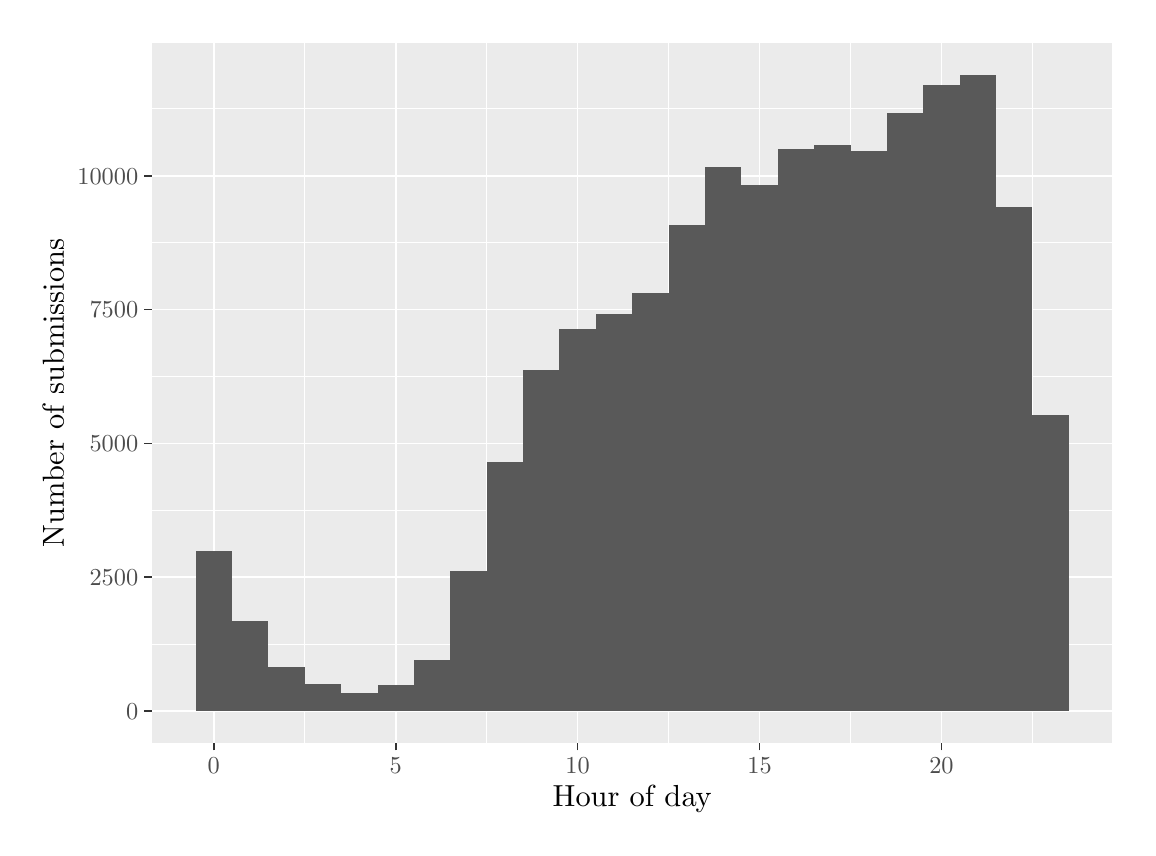
\begin{tikzpicture}[x=1pt,y=1pt]
\definecolor{fillColor}{RGB}{255,255,255}
\path[use as bounding box,fill=fillColor,fill opacity=0.00] (0,0) rectangle (397.48,289.08);
\begin{scope}
\path[clip] (  0.00,  0.00) rectangle (397.48,289.08);
\definecolor{drawColor}{RGB}{255,255,255}
\definecolor{fillColor}{RGB}{255,255,255}

\path[draw=drawColor,line width= 0.6pt,line join=round,line cap=round,fill=fillColor] (  0.00,  0.00) rectangle (397.48,289.08);
\end{scope}
\begin{scope}
\path[clip] ( 44.91, 30.69) rectangle (391.98,283.58);
\definecolor{fillColor}{gray}{0.92}

\path[fill=fillColor] ( 44.91, 30.69) rectangle (391.98,283.58);
\definecolor{drawColor}{RGB}{255,255,255}

\path[draw=drawColor,line width= 0.3pt,line join=round] ( 44.91, 66.35) --
	(391.98, 66.35);

\path[draw=drawColor,line width= 0.3pt,line join=round] ( 44.91,114.70) --
	(391.98,114.70);

\path[draw=drawColor,line width= 0.3pt,line join=round] ( 44.91,163.04) --
	(391.98,163.04);

\path[draw=drawColor,line width= 0.3pt,line join=round] ( 44.91,211.38) --
	(391.98,211.38);

\path[draw=drawColor,line width= 0.3pt,line join=round] ( 44.91,259.73) --
	(391.98,259.73);

\path[draw=drawColor,line width= 0.3pt,line join=round] (100.13, 30.69) --
	(100.13,283.58);

\path[draw=drawColor,line width= 0.3pt,line join=round] (165.86, 30.69) --
	(165.86,283.58);

\path[draw=drawColor,line width= 0.3pt,line join=round] (231.59, 30.69) --
	(231.59,283.58);

\path[draw=drawColor,line width= 0.3pt,line join=round] (297.33, 30.69) --
	(297.33,283.58);

\path[draw=drawColor,line width= 0.3pt,line join=round] (363.06, 30.69) --
	(363.06,283.58);

\path[draw=drawColor,line width= 0.6pt,line join=round] ( 44.91, 42.18) --
	(391.98, 42.18);

\path[draw=drawColor,line width= 0.6pt,line join=round] ( 44.91, 90.52) --
	(391.98, 90.52);

\path[draw=drawColor,line width= 0.6pt,line join=round] ( 44.91,138.87) --
	(391.98,138.87);

\path[draw=drawColor,line width= 0.6pt,line join=round] ( 44.91,187.21) --
	(391.98,187.21);

\path[draw=drawColor,line width= 0.6pt,line join=round] ( 44.91,235.56) --
	(391.98,235.56);

\path[draw=drawColor,line width= 0.6pt,line join=round] ( 67.26, 30.69) --
	( 67.26,283.58);

\path[draw=drawColor,line width= 0.6pt,line join=round] (132.99, 30.69) --
	(132.99,283.58);

\path[draw=drawColor,line width= 0.6pt,line join=round] (198.73, 30.69) --
	(198.73,283.58);

\path[draw=drawColor,line width= 0.6pt,line join=round] (264.46, 30.69) --
	(264.46,283.58);

\path[draw=drawColor,line width= 0.6pt,line join=round] (330.19, 30.69) --
	(330.19,283.58);
\definecolor{fillColor}{gray}{0.35}

\path[fill=fillColor] ( 60.69, 42.18) rectangle ( 73.83,100.02);

\path[fill=fillColor] ( 73.83, 42.18) rectangle ( 86.98, 74.63);

\path[fill=fillColor] ( 86.98, 42.18) rectangle (100.13, 58.15);

\path[fill=fillColor] (100.13, 42.18) rectangle (113.27, 51.91);

\path[fill=fillColor] (113.27, 42.18) rectangle (126.42, 48.50);

\path[fill=fillColor] (126.42, 42.18) rectangle (139.57, 51.71);

\path[fill=fillColor] (139.57, 42.18) rectangle (152.71, 60.47);

\path[fill=fillColor] (152.71, 42.18) rectangle (165.86, 92.63);

\path[fill=fillColor] (165.86, 42.18) rectangle (179.01,132.04);

\path[fill=fillColor] (179.01, 42.18) rectangle (192.15,165.40);

\path[fill=fillColor] (192.15, 42.18) rectangle (205.30,180.21);

\path[fill=fillColor] (205.30, 42.18) rectangle (218.45,185.74);

\path[fill=fillColor] (218.45, 42.18) rectangle (231.59,193.07);

\path[fill=fillColor] (231.59, 42.18) rectangle (244.74,217.86);

\path[fill=fillColor] (244.74, 42.18) rectangle (257.89,238.86);

\path[fill=fillColor] (257.89, 42.18) rectangle (271.03,232.11);

\path[fill=fillColor] (271.03, 42.18) rectangle (284.18,245.32);

\path[fill=fillColor] (284.18, 42.18) rectangle (297.33,246.77);

\path[fill=fillColor] (297.33, 42.18) rectangle (310.47,244.49);

\path[fill=fillColor] (310.47, 42.18) rectangle (323.62,258.30);

\path[fill=fillColor] (323.62, 42.18) rectangle (336.77,268.49);

\path[fill=fillColor] (336.77, 42.18) rectangle (349.92,272.08);

\path[fill=fillColor] (349.92, 42.18) rectangle (363.06,224.40);

\path[fill=fillColor] (363.06, 42.18) rectangle (376.21,148.98);
\end{scope}
\begin{scope}
\path[clip] (  0.00,  0.00) rectangle (397.48,289.08);
\definecolor{drawColor}{gray}{0.30}

\node[text=drawColor,anchor=base east,inner sep=0pt, outer sep=0pt, scale=  0.88] at ( 39.96, 39.15) {0};

\node[text=drawColor,anchor=base east,inner sep=0pt, outer sep=0pt, scale=  0.88] at ( 39.96, 87.49) {2500};

\node[text=drawColor,anchor=base east,inner sep=0pt, outer sep=0pt, scale=  0.88] at ( 39.96,135.84) {5000};

\node[text=drawColor,anchor=base east,inner sep=0pt, outer sep=0pt, scale=  0.88] at ( 39.96,184.18) {7500};

\node[text=drawColor,anchor=base east,inner sep=0pt, outer sep=0pt, scale=  0.88] at ( 39.96,232.53) {10000};
\end{scope}
\begin{scope}
\path[clip] (  0.00,  0.00) rectangle (397.48,289.08);
\definecolor{drawColor}{gray}{0.20}

\path[draw=drawColor,line width= 0.6pt,line join=round] ( 42.16, 42.18) --
	( 44.91, 42.18);

\path[draw=drawColor,line width= 0.6pt,line join=round] ( 42.16, 90.52) --
	( 44.91, 90.52);

\path[draw=drawColor,line width= 0.6pt,line join=round] ( 42.16,138.87) --
	( 44.91,138.87);

\path[draw=drawColor,line width= 0.6pt,line join=round] ( 42.16,187.21) --
	( 44.91,187.21);

\path[draw=drawColor,line width= 0.6pt,line join=round] ( 42.16,235.56) --
	( 44.91,235.56);
\end{scope}
\begin{scope}
\path[clip] (  0.00,  0.00) rectangle (397.48,289.08);
\definecolor{drawColor}{gray}{0.20}

\path[draw=drawColor,line width= 0.6pt,line join=round] ( 67.26, 27.94) --
	( 67.26, 30.69);

\path[draw=drawColor,line width= 0.6pt,line join=round] (132.99, 27.94) --
	(132.99, 30.69);

\path[draw=drawColor,line width= 0.6pt,line join=round] (198.73, 27.94) --
	(198.73, 30.69);

\path[draw=drawColor,line width= 0.6pt,line join=round] (264.46, 27.94) --
	(264.46, 30.69);

\path[draw=drawColor,line width= 0.6pt,line join=round] (330.19, 27.94) --
	(330.19, 30.69);
\end{scope}
\begin{scope}
\path[clip] (  0.00,  0.00) rectangle (397.48,289.08);
\definecolor{drawColor}{gray}{0.30}

\node[text=drawColor,anchor=base,inner sep=0pt, outer sep=0pt, scale=  0.88] at ( 67.26, 19.68) {0};

\node[text=drawColor,anchor=base,inner sep=0pt, outer sep=0pt, scale=  0.88] at (132.99, 19.68) {5};

\node[text=drawColor,anchor=base,inner sep=0pt, outer sep=0pt, scale=  0.88] at (198.73, 19.68) {10};

\node[text=drawColor,anchor=base,inner sep=0pt, outer sep=0pt, scale=  0.88] at (264.46, 19.68) {15};

\node[text=drawColor,anchor=base,inner sep=0pt, outer sep=0pt, scale=  0.88] at (330.19, 19.68) {20};
\end{scope}
\begin{scope}
\path[clip] (  0.00,  0.00) rectangle (397.48,289.08);
\definecolor{drawColor}{RGB}{0,0,0}

\node[text=drawColor,anchor=base,inner sep=0pt, outer sep=0pt, scale=  1.10] at (218.45,  7.64) {Hour of day};
\end{scope}
\begin{scope}
\path[clip] (  0.00,  0.00) rectangle (397.48,289.08);
\definecolor{drawColor}{RGB}{0,0,0}

\node[text=drawColor,rotate= 90.00,anchor=base,inner sep=0pt, outer sep=0pt, scale=  1.10] at ( 13.08,157.13) {Number of submissions};
\end{scope}
\end{tikzpicture}
